%!TEX root = ../main.tex

\section{Fainder}
\label{sec:index_overview}

We propose \system{}, an index for percentile predicates that attains robust scalability and accurate (optionally exact) results to address the identified research challenges.
This section gives an overview of \system{}'s architecture.
Subsequently, we discuss the technical details of index construction and querying in Sections~\ref{sec:index_construction} and~\ref{sec:index_querying}.

\paragraph{Key Insights}
The central intuition behind \system{} is that whenever all histograms have the same set of bins, we can precompute a subset of cumulative densities to answer percentile predicates efficiently with sublinear time complexity.
Conceptually, we achieve a logarithmic scaling by sorting the histograms' cumulative densities at each bin boundary and using a two-stage binary search over the bins and densities to identify the result set.
In practice, however, histogram heterogeneity prevents us from directly using binary search on a collection.
To overcome this limitation, \system{} homogenizes histograms by mapping them to a collection-wide consistent bin distribution.
Changing the bin edges of a histogram and reassigning a bin's density to one or multiple new bins is inherently approximate.
Thus, we must ensure that \system{} has high accuracy comparable to \pscan during index construction.
Naive approaches to creating such a global distribution are constructing the union of all original bin edges or creating $\epsilon$-sized bins between the minimum and maximum value of a collection.
However, these approaches lead to an excessive memory footprint or subpar result accuracy, as we show with a concrete example in Section~\ref{sec:clustering}.
\system{} addresses these challenges by creating a clustered global bin distribution instead.
Empirical evaluation on one million datasets (GitTables~\cite{hulsebos_gittables_2023}) shows that our clustering approach reduces the memory footprint from more than one TB to 3.2 GB without a substantial increase in runtime while maintaining high accuracy.

\paragraph{System Overview}

\begin{figure}[t]
    \centering
    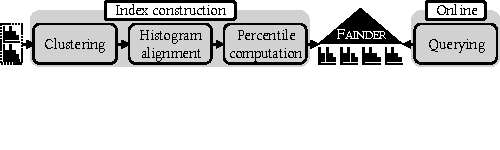
\includegraphics[trim=0 1.4cm 0 0]{figures/diagrams/fainder.pdf}
    \caption{Overview of \system{}.}
    \Description{Schematic system overview that describes the different stages of \system{}.}
    \label{fig:fainder_overview}
    % Max width: 241.14749pt / 8.47cm
\end{figure}

Figure~\ref{fig:fainder_overview} summarizes the lifecycle of \system{}.
The starting point is a histogram collection $\cH$ and a mapping $\FuncSty{column}(H)$ that projects each histogram to its associated column identifier.
At first, \system{} clusters $\cH$ based on the bin edges of each histogram.
As part of the clustering phase, we must decide what share of the global bin budget (i.e.,~memory budget) we assign to each cluster and how the bin edges within a cluster should be distributed.
Next, \system{} aligns the histograms $\cH_c$ in a cluster $c$ by distributing the original bin density $\density{H}$ to $\density{H'}$ based on the cluster bins $\edges{\cH_c}$.
For this, we introduce two alternative histogram alignment techniques, rebinning and conversion, that offer different trade-offs for precision, recall, and index size.
Having aligned all histograms in a cluster, \system{} indexes them by precomputing and sorting the cumulative density per histogram and bin.
Finally, \system{} evaluates percentile predicates using binary search at query time.
Like any search index, \system{} amortizes its additional memory consumption and one-time construction cost through repeated execution time savings each time it evaluates a predicate.
We discuss the conceptual index maintenance costs in Section~\ref{sec:percentile_computation} and experimentally evaluate them in Section~\ref{sec:micro_benchmarks}.\looseness=-1

\paragraph{Index Variants}

\begin{figure}[t]
    \centering
    \begin{forest}
    forked edges,
    for tree={
        font=\scriptsize,
        draw,
        rounded corners=2pt,
        align=center,
        inner sep=2pt,
        edge={font=\scriptsize, -stealth},
        calign=center,
        l sep=0.1em,
        s sep-=1pt,
        fork sep=0.5em,
    }
    [{Do you require exact query results?}
        [{Do you have a tight memory budget?}, edge label={node[midway,left] {No}}
            [{Use \approximate{} with\\rebinning-based alignment.}, edge label={node[midway,left] {Yes}}, tier=rec]
            [{Use \approximate{} with\\conversion-based alignment.}, edge label={node[midway,right] {No}}, tier=rec]
        ]
        [{Use \exact{} with\\conversion-based alignment.}, edge label={node[midway,right] {Yes}}, tier=rec]
    ]
    \end{forest}
    \caption{Flowchart for choosing a \system{} variant.}
    \Description{Questions for choosing a \system{} variant.}
    \label{fig:index_variants}
\end{figure}

The two histogram alignment techniques enable us to design three unique \system{} variants that cater to different requirements.
Figure~\ref{fig:index_variants} summarizes them with guidelines for choosing an appropriate version.
If exact results are not required or execution time is paramount, rebinning and conversion offer two alternative \approximate{} variants.
While rebinning minimizes the index size and construction time, conversion allows users to select a full precision or recall guarantee at query time.
Thus, \exact{} utilizes a conversion-based index to efficiently prune the search space before conducting \pscan on a small subset of histograms.
Note that a conversion-based index can be used for both approximate and exact results based on the runtime preference per query.
Therefore, the primary decision during index construction is to choose either rebinning- or conversion-based histogram alignment.\looseness=-1


\section{Index Construction}
\label{sec:index_construction}

We discuss the construction of \system{}, which consists of the steps clustering, histogram alignment, and percentile computation.\looseness=-1

\subsection{Clustering}
\label{sec:clustering}

The clustering phase computes a feature vector for each histogram, clusters them, and defines the aligned bins for each cluster.
The motivation for this phase are the bin width and value range differences between histograms in a dataset collection.
To illustrate this, consider the histogram collection from Figure~\ref{fig:example_histograms_2}, which we use as a running example throughout this section, and assume that there is another histogram $H_5$ with $\edges{H_5} = [-100, -85, -70]$ (not depicted for brevity).
The global value range of this collection is [-100, 100].
However, no histogram covers the interval (-70, 0).
Therefore, allocating bins in the global bin distribution for this region would be a waste of space, as there are no density changes.
Furthermore, $H_1$ and $H_4$ both cover the interval [0, 3] but with vastly different bin widths.
Thus, converting $\edges{H_1}$ and $\edges{H_4}$ to a joint bin distribution would be too detailed for $H_1$ or too coarse for $H_4$.
Considering that \system{} should have a minimal memory footprint, aligned bins must only cover relevant parts of the global value range with a locally appropriate bin width to achieve accurate query responses efficiently.
Since we do not know user queries in advance, an optimal solution is query-agnostic and minimizes the information loss between original and global bins, given a user-defined bin budget $\cB$.
Formally, we consider the overlap of each original bin $b_i \equiv [b_{il}, b_{ih})$ with the closest global bin $b_j^g$ as a proxy for mitigating information loss and thus aim to maximize it:
\begin{equation}
\label{eq:overlap_optimization}
\underset{b^g}{\FuncSty{argmax }} O = \mathcolor{brown!80}{\sum_{i}} \mathcolor{red!70}{\underset{j}{\FuncSty{max}}} \left( \frac{\mathcolor{red!70}{\FuncSty{max} \left(\FuncSty{min}(b^{}_{ih}, b^g_{jh}) - \FuncSty{max}(b^{}_{il}, b^g_{jl}), 0\right)}}{\mathcolor{blue!70}{\FuncSty{max}\left(\FuncSty{width}(b_i), \FuncSty{width}(b_j^g)\right)}} \right)
\end{equation}
The cumulative overlap $O$ reflects the overlap between an original bin and the most closely fitting global bin (red), normalized by the bin width (blue), and summed across original bins (brown).
If we consider each possible global bin as a unit-weight item whose value is its marginal improvement of $O$, finding an optimal solution with a limited number of bins is a variation of the knapsack problem (i.e.,~NP-hard).
Therefore, we use a three-step procedure based on clustering to break down the global bin definition problem into smaller parts and efficiently find an approximate solution.

\begin{figure}[t]
    \centering
    \begin{tikzpicture}
        \node(H1) {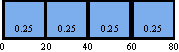
\includegraphics[page=1, scale=1]{figures/diagrams/histograms.pdf}};
        \node(H2) [right=15mm of H1.south east, anchor=south west] {\includegraphics[page=3, scale=1]{figures/diagrams/histograms.pdf}};
        \node(H3) [below=0mm of H1.south west, anchor=north west] {\includegraphics[page=4, scale=1]{figures/diagrams/histograms.pdf}};
        \node(H4) [right=15mm of H3.south east, anchor=south west] {\includegraphics[page=2, scale=1]{figures/diagrams/histograms.pdf}};

        \node[left=0mm of H1, inner sep=0mm] {$H_1$};
        \node[left=0mm of H2, inner sep=0mm] {$H_2$};
        \node[left=0mm of H3, inner sep=0mm] {$H_3$};
        \node[left=3mm of H4, inner sep=0mm] {$H_4$};

        \node [bound, fit margins = {left=9pt,right=3pt, bottom=0pt,top=5pt}, fit=(H1) (H3)] {$\cH_1$};
        \node [bound, fit margins = {left=9pt,right=2pt, bottom=0pt,top=0pt}, fit=(H2) (H4)] {$\cH_2$};
    \end{tikzpicture}
    \caption{Histograms $H_1$--$H_4$ and clusters $\cH_1, \cH_2$.}
    \Description{A set of four example histograms used throughout Section~\ref{sec:index_construction}.}
    \label{fig:example_histograms_2}
    \vspace{0.6em}
\end{figure}

\paragraph{Clustering Features}
Clustering aims to partition the histogram collection $\cH$ into sets of histograms that cover similar value ranges with similar bin widths.
Therefore, we compute a feature vector
\[
\boldsymbol{v}_{H} = \begin{bmatrix}\FuncSty{min}(\edges{H}) & \FuncSty{max}(\edges{H}) & \FuncSty{avgWidth}(\edges{H})\end{bmatrix}
\]
for each histogram, where \FuncSty{avgWidth} represents the average bin width of a histogram.
Due to the heterogeneity of histograms, directly clustering the feature vectors would yield suboptimal results.
Therefore, we preprocess them with a non-linear quantile transform~\cite{pedregosa_scikit-learn_2011}, which maps all features to a uniform distribution on the interval $[0, 1]$ to reduce the impact of outliers.
The intuition for this transformation is to make the different value scales of our features more directly comparable while being robust to outliers.

\paragraph{Clustering Algorithm}
\system{} requires a scalable clustering algorithm to partition all histograms into reasonable, ideally balanced clusters.
Conceptually, the clustering algorithm choice is a hyperparameter of \system{} and orthogonal to the other stages.
Concretely, we use k-Means~\cite{lloyd_least_1982} for clustering and discuss our investigation of alternative clustering algorithms in Section~\ref{sec:solution_effectiveness}.

\paragraph{Cluster Bin Assignment}

\begin{figure}[t]
    \begin{tikzpicture}
        \node(H13) {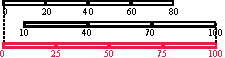
\includegraphics[page=1]{figures/diagrams/fainder_overview.pdf}};
        \node(H1) [above left=-4mm and -2mm of H13] {\small $H_1$};
        \node(H2) [below=-0.8mm of H1] {\small $H_3$};
        \node(CH1) [below=-0.8mm of H2] {\small $\cH_1$};

        \node(H24) [right = 5mm of H13] {\includegraphics[page=4]{figures/diagrams/fainder_overview.pdf}};
        \node(H4) [above left=-4mm and -2mm of H24] {\small $H_4$};
        \node(H2) [below=-0.8mm of H4] {\small $H_2$};
        \node(CH2) [below=-0.8mm of H2] {\small $\cH_2$};
    \end{tikzpicture}
    \caption{Cluster bin assignment for $\cH_1$ and $\cH_2$ ($\cB=8$).}
    \Description{A visual summary of histogram clustering based on the histogram bin edges and subsequent cluster bin assignment.}
    \label{fig:bin_assignment}
\end{figure}

\begin{figure}[t]
    \subfloat[$H_1 \to H'_1$]{
        \includegraphics[page=2]{figures/diagrams/fainder_overview.pdf}
    }%
    \hfill%
    \subfloat[$H_2 \to H'_2$]{
        \includegraphics[page=6]{figures/diagrams/fainder_overview.pdf}
    }

    \subfloat[$H_3 \to H'_3$]{
        \includegraphics[page=3]{figures/diagrams/fainder_overview.pdf}
    }%
    \hfill%
    \subfloat[$H_4 \to H'_4$]{
        \includegraphics[page=5]{figures/diagrams/fainder_overview.pdf}
    }
    \caption{Rebinning-based histogram alignment. The aligned histogram bins and densities are shown in red.}
    \Description{An example of the rebinning procedure based on the histograms from Figure~\ref{fig:example_histograms_2} and cluster bins from Figure~\ref{fig:bin_assignment}.}
    \label{fig:rebinning_alignment}
\end{figure}

After clustering, we must distribute the global bin budget $\cB$ across clusters.
Figure~\ref{fig:bin_assignment} demonstrates this final step of the clustering phase with our running example.
The simplest method is to assign a budget proportional to the cluster size:\looseness=-1
\begin{equation}
\label{eq:cluster_bin_budget}
\cB_c =  \FuncSty{max}\left(1, \left\lfloor \cB \frac{|\cH_c|}{\sum_{i=1}^k |\cH_i|} \right\rfloor \right)
\end{equation}
However, in the worst case, this results in small clusters only consisting of a single bin, whereas large clusters might receive a much more fine-grained bin width than needed.
Therefore, we use additive smoothing~\cite{manning_introduction_2008} to anneal the proportional bin budget towards a uniform assignment based on the parameter $\alpha$.
Given a cluster (value range) and bin budget, we create equi-width bins $\edges{\cH_c}$ for each cluster.
Conceptually, the cluster bin assignment strategy is a hyperparameter that a search engine operator can adapt.
For example, we could instead allocate the same bin budget to each cluster or choose an individual bin definition algorithm for each cluster, such as equi-height bins (which are more costly to compute).


\subsection{Histogram Alignment}
\label{sec:alignment}

Given a cluster of histograms $\cH_c$ and its cluster bins $\edges{\cH_c}$, the task of histogram alignment is to transform each $H \in \cH_c$ to $H'$, such that $\density{H'}$ represents the original value distribution of $H$ on $\edges{\cH_c}$.
This requires distributing the density of each original bin to one or multiple new bins.
Consequently, histogram alignment requires approximating the data distribution within a bin and strongly influences the downstream index accuracy.

We present two alternative approaches for histogram alignment that offer different trade-offs between index accuracy and resource requirements.
Rebinning aims to minimize the index size but does not provide a formal accuracy guarantee.
It allows the system operator to make an assumption about the intra-bin value distribution and will balance precision and recall if the assumption holds.
While rebinning is an intuitive and efficient way to align histograms, there are scenarios where guaranteeing total precision or recall is critical.
For example, precision is essential if users only want to review a few guaranteed true results.
Contrarily, total recall is crucial to use \system{} as a pruning tool for an exact solution.
Thus, conversion ensures total recall or precision at query time but requires additional storage compared to rebinning.

\paragraph{Rebinning}
The principal idea of rebinning is to compute the overlap interval $o_{ij} = [\FuncSty{max}(b_{il}, b_{jl}), \FuncSty{min}(b_{ih}, b_{jh}))$ between all pairs of bins $b_i$ from the original histogram and $b_j$ from the respective cluster bins.
Given $o_{ij}$, we compute the fraction of the original bin's density $\density{H}[i]$ that lies within $o_{ij}$ and add it to $\density{H'}[j]$.
Since a histogram does not contain information about the distribution of values within a bin, rebinning must approximate this fraction if $o_{ij} \neq b_i$.
The simplest intra-bin density estimation assumes a uniform value distribution within a bin (i.e.,~we add $\tfrac{\FuncSty{width}(o_{ij})}{\FuncSty{width}(b_i)}\%$ of $b_i$'s density to $b_j$)~\cite{cormode_synopses_2011}.
However, a search engine can make other assumptions about the data distribution.
For instance, cubic spline interpolation is a more costly alternative but can better estimate non-uniform value distributions.

Figure~\ref{fig:rebinning_alignment} continues our running example and shows how to rebin $H_1$--$H_4$ based on the cluster bins.
For example, the fourth bin of $H_2$ has the range $[5,\;8]$.
Thus, its overlap with $\cH_2[2]$ is $o_{32} = [5,\;6)$.
Under a continuous value assumption, this means that one-third of $H_2[3]$'s density (0.1) is assigned to $\density{H'_2}[2]$, which, together with the contributions from $H_2[2]$, has a total density of 0.3.

\paragraph{Conversion}

The central intuition of conversion-based histogram alignment is to compute a lower and upper bound for the density at each bin.
To compute these bounds, we create a \textit{conversion matrix} $CM$ for every array pair ($\edges{H}$, $\edges{\cH_c}$) of original bins and cluster bins.
$CM$ is a Boolean matrix that is true for each bin pair that partially or fully overlaps.
Based on $CM$, we know which original bin \textit{might} or \textit{must} contribute to the density of any bin in $H'$.
Since the original and cluster bins form an n:m relationship, we cannot assume that the upper bound of $H'[i]$ is the lower bound of $H'[i+1]$.
This requires us to store two numbers per bin, resulting in a $2\times$ index size compared to rebinning.
At the same time, conversion enables predicate evaluation with full precision or recall, as we do not perform any intra-bin estimation but fully add $\density{H}[i]$ to $\density{H'}[j]$ if it contributes to the lower or upper bound of the bin's density.
Depending on the comparison operator in a predicate, \system{} uses the respective density bound to prevent false positives or negatives.
Given a query, such as ``at least 50\% of the values are lower than 60'' with a total recall requirement, the upper density bound lets us filter out those histograms that do not have a cumulative density higher than 50\% in the bin where 60 lies.

Figure~\ref{fig:conversion_alignment} shows the conversion matrix for histogram $H_2$ and cluster $\cH_2$ on the left.
On the right, we visualize the bin-wise conversion of $H_2$.
In practice, we do not convert each bin separately but directly compute the lower and upper bounds for the cumulative density of a bin.
By knowing which cluster bins an original bin partially contributes to, we also know that this bin must fully contribute to the cumulative density of all following cluster bins, highlighted by the green lower bound area.
The orange upper bound area consists of the lower bound area and the bins whose contribution is unclear.
We compute the cumulative bounds by summing up the density of all original bins that contribute to a cluster bin's lower or upper bound.
The cumulative density of $H'_2[2]$, for example, is bounded by $[0.5,\:1]$ since the first two bins of $H_2$ (green area) fully contribute to the bin's density.
In contrast, the orange area (bins 1-4) comprises the original bins that might contribute to the cumulative density of $H'_2[2]$.\looseness=-1

\begin{figure}[t]
    \begin{tikzpicture}[anchor=north west, every node/.style={font=\scriptsize}]
        \matrix(mat) [
        nodes=draw,minimum width=6mm,
        column sep=0mm,
        font=\small,
        ]
        {
        \node(11) {1};   & \node(12){1};     & \node(13){0};      & \node(14){0}; \\
        \node(21) {0};   & \node(22){1};     & \node(23){0};      & \node(24){0}; \\
        \node(31) {0};   & \node(33){0};     & \node(33){1};      & \node(34){0}; \\
        \node(41) {0};   & \node(42){0};     & \node(43){1};      & \node(44){1}; \\
        };

        \begin{pgfonlayer}{background}
        \foreach \x in {11,12,13,14,22,23,24,33,34,43,44}
        \filldraw[DarkOrange!60][] ($(\x.north west)+(0.1ex, -0.1ex)$) -- ($(\x.south west)+(0.1ex, 0.1ex)$) -- ($(\x.south east)+(-0.1ex, 0.1ex)$)--cycle;

        \foreach \x in {13,14,23,24,34}
        \filldraw[ForestGreen!60][] ($(\x.north west)+(0.2ex, -0.1ex)$) -- ($(\x.north east)+(-0.1ex, -0.1ex)$) -- ($(\x.south east)+(-0.1ex, 0.15ex)$)--cycle;
        \end{pgfonlayer}

        \node[left=8mm of mat, rotate=90, anchor=north] {$\edges{H_2}$};
        \node[above=1.5mm of mat] {$\edges{\cH_2}$};

        \node[above=0mm of 11] {[0,2)};
        \node[above=0mm of 12] {[2,4)};
        \node[above=0mm of 13] {[4,6)};
        \node[above=0mm of 14] {[6,8]};

        \node[left=0mm of 11] {[1,3)};
        \node[left=0mm of 21] {[3,4)};
        \node[left=0mm of 31] {[4,5)};
        \node[left=0mm of 41] {[5,8]};

        \node(H2)[right=1mm of mat.south east, anchor=south west] {\includegraphics[page=9]{figures/diagrams/fainder_overview.pdf}};

        \node[below=-1mm of mat] {$CM(H_2, \cH_2)$};
        \node[below=-1mm of H2] {$H_2 \to H'_2$};

        \node[draw, fill=DarkOrange!60, minimum width=1mm, left=12mm of mat.south west, anchor=south] (ub) {};
        \node[draw, fill=ForestGreen!60, minimum width=1mm, left=2mm of ub.south west, anchor=south] (lb) {};
        \node[above=0.5mm of lb.north, anchor=west, rotate=90] {\scriptsize\itshape Lower bound};
        \node[above=0.5mm of ub.north, anchor=west, rotate=90] (ubtext) {\scriptsize\itshape Upper bound};
        \node[draw, dashed, fit margins = {left=1pt,right=0pt,bottom=1pt,top=1pt}, fit=(lb)(ubtext)] {};
    \end{tikzpicture}
    \captionsetup{belowskip=0.0em, aboveskip=-0.3em}
    \caption{Conversion-based histogram alignment: (left) conversion matrix for computing percentile bounds, (right) aligned histogram with lower and upper bounds in red.}
    \Description{An example of the conversion procedure based on histogram $H_2$ from the example histograms.}
    \label{fig:conversion_alignment}
    \vspace{-0.3em}
\end{figure}

\subsection{Percentile Computation}
\label{sec:percentile_computation}

\begin{figure}[t]
    \centering
    \begin{tikzpicture}
        \node(H1) {\includegraphics[page=7,scale=0.86]{figures/diagrams/fainder_overview.pdf}};
        \node(H2) [right=1.5mm of H1.north east, anchor=north west] {\includegraphics[page=8,scale=0.86]{figures/diagrams/fainder_overview.pdf}};
        \node [bound, fit margins = {left=-1pt,right=-1pt, bottom=0pt,top=-1pt}, fit=(H1), label={[anchor=south west, inner sep=2pt, text=gray]south west:$\cH_1$}] {};
        \node [bound, fit margins = {left=-1pt,right=-1pt, bottom=0pt,top=-1pt}, fit=(H2), label={[anchor=south east, inner sep=2pt, text=gray]south east:$\cH_2$}] {};

        \path (H1.north) -- (H2.north) node[inner sep=1pt, yshift=2pt, midway] (ab) {\scriptsize\itshape Aligned bin edges};
        \path (H1.east) -- (H2.west) node[inner sep=1pt, yshift=-12pt, midway] (cd) {\scriptsize\itshape Cumulative densities};

        \draw[-, thick] (H1.north) |- (ab) -| (H2.north);
        \draw[-, thick] ([yshift=-7pt]H1.center) |- (cd) -| ([yshift=-7pt]H2.center);
        \draw[-, thick] ([yshift=8pt, xshift=30pt]H1.south) -- node[inner sep=1pt, fill=white]{\scriptsize\itshape Histogram pointers} ([yshift=8pt, xshift=-30pt]H2.south);
    \end{tikzpicture}
    \caption{Rebinning-based \system{} index for $H_1$--$H_4$. Red color outlines evaluating the predicate \textit{``at least 65\% of the values are less than 50''}. Dashed arrows are histogram pointers.\looseness=-1}
    \Description{A visualization of index construction and querying.}
    \label{fig:percentile_computation_and_querying}
    \vspace{-0.4em}
\end{figure}

The percentile computation phase consists of initialization, density summation, and sorting.
We demonstrate its result in the upper part of Figure~\ref{fig:percentile_computation_and_querying}.
For each cluster $c$, \system{} creates a $(n_c \times \cB_c)$ array to store percentiles and a pointer array of the same size to keep a reference to the respective histograms.
For conversion-based indices, this array pair is created twice for the lower and upper percentile bounds.
Next, \system{} computes the cumulative density per cluster bin and histogram.
Since all histograms in a cluster have the same bins, \system{} uses vectorization to compute the cumulative sums efficiently and stores them in the percentile array.
Lastly, we sort the percentile array and corresponding pointers column-wise.
This way, \system{} knows that all histogram pointers after a given one in the current bin have an equal or higher cumulative density.\looseness=-1

\paragraph{Index Size and Maintenance Costs}
\system{}'s query execution time improvements must justify its overhead, specifically the memory consumption and maintenance cost.
Without clustering, \system{}'s asymptotic space complexity is $O(n \cB)$, as we must store a percentile-pointer pair for each histogram and global bin.
However, with clustering, we do not have to process the full Cartesian product of histograms and bins across clusters, making construction faster and the index smaller.
The more clusters an index has, and the more evenly balanced they are, the smaller the size of \system{}.
In the case of a perfectly even distribution, the size shrinks to $O(\frac{n \cB}{k})$.

The maintenance costs of \system{} are divided into one-time construction costs and repeated histogram insertion and deletion costs.
Since we have to initially cluster and individually align each histogram, the construction costs scale linearly with $n$.
However, these costs are mitigated by the fact that an index is seldom created but often queried.
More importantly, we can insert into and delete from \system{} at minimal cost since histogram alignment is an incremental process as long as we do not change the cluster bins and assign new histograms to existing clusters.


\section{Index Querying}
\label{sec:index_querying}

We discuss using \system{}'s design for fast and accurate percentile predicate evaluation.
Our index offers two query modes, \approximate{} and \exact{}, which we delineate in this section.

\subsection{\approximate{}}
\label{sec:approx_query}

\begin{algorithm}[t]
    \caption{Percentile predicate evaluation with \system{}.}
    \label{alg:index_query}
    \KwIn{index $\cI$, cluster bins $\sset{\edges{\cH_c}}_{c=1}^k$, predicate $\cP$}
    \KwOut{Solution set $S$}

    $C, p, \theta, r_h \gets \cP$, $S \gets \{\;\}$, $l \gets 0$\;
    \lIf{$\theta \in \{<, \leq\}$}{
        $l \gets 1$ \tcp*[f]{Upper bound for ``at least'' predicates}
    }
    \For{$c \gets 1$ \KwTo $k$}{
        \If{$\FuncSty{min}(\edges{\cH_c}) \leq r_h \leq \FuncSty{max}(\edges{\cH_c})$}{
            $i \gets \FuncSty{binarySearch}(\edges{\cH_c}, r_h)$ \tcp*[r]{Bin index $i$} \label{alg:bin_index_search}
            $j \gets \FuncSty{binarySearch}(\cI_{cl}^P[:, i], p)$ \tcp*[r]{Histogram index $j$} \label{alg:hist_index_search}
            \If(\tcp*[f]{``at least'' predicate}){$\theta \in \{<, \leq\}$}{
                $S \gets S \cup \cI_{cl}^H[j:, i]$ \tcp*[r]{Include all rows after $j$} \label{alg:add_after}
            }
            \Else(\tcp*[f]{``at most'' predicate}){
                $S \gets S \cup \cI_{cl}^H[:j, i]$ \tcp*[r]{Include all rows before $j$} \label{alg:add_before}
            }
        }
        \Else(\tcp*[f]{$r_h$ not in cluster range}){
            \If{$(r_h \leq \FuncSty{min}(\edges{\cH_c}) \wedge \theta \in \{>, \geq\}) \; \vee$ \\
                \nonl\mbox{}\phantom{\KwSty{if} }$(r_h \geq \FuncSty{max}(\edges{\cH_c}) \wedge \theta \in \{<, \leq\})$}{ \label{alg:cluster_skip}
                $S \gets S \cup \cI_{cl}^H$ \tcp*[r]{Add all pointers from cluster} \label{alg:after_cluster}
            }
        }
    }
    \ForEach{$s \in S$}{
        \lIf{$\FuncSty{column}(s) \notin C$}{
            $S \gets S - s$
        }
    }
    \Return S\;
\end{algorithm}

The approximate version of our index is designed to minimize runtime while offering two different approaches to trade off resource efficiency and accuracy guarantees.
Algorithm~\ref{alg:index_query} shows the query procedure for a conversion-based index with full recall guarantees.
Formally, \system{} is a data structure $\cI\equiv (\cI^P, \cI^H)$ that consists of percentile and histogram pointer arrays.
We use $\cI_{cl}$ to denote the cluster $c \in \{1, \ldots, k\}$ and the lower or upper percentile limit $l \in \{0, 1\}$.
\system{} first decides which bound to use based on the predicate's comparison operator $\theta$.
For a rebinning-based index, $l$ is always 0.
Then, it iterates through each index cluster $c$.
If the query's range value $r_h$ does not fall into the range of a cluster, \system{} adds either all or no histograms from the cluster to $S$, depending on $\theta$ and whether $r_h$ lies above or below the cluster range.
Otherwise, \system{} first performs binary search to identify which cluster bin $r_h$ falls into (line~\ref{alg:bin_index_search}).
Then, it conducts another binary search within that bin to identify the first (for ``at least'' predicates) or last (for ``at most'') histogram that matches $p$ (line~\ref{alg:hist_index_search}).
Finally, it adds the histogram pointer from the identified cell and all following (``at least'', line~\ref{alg:add_after}) or preceding (``at most'', line~\ref{alg:add_before}) pointers from the column to $S$.
The query procedures for re\-bin\-ning- or con\-ver\-sion-ba\-sed indices with total precision differ from Algorithm~\ref{alg:index_query} in a few conditional statements that we omit for improved readability.\looseness=-1

Figure~\ref{fig:percentile_computation_and_querying} concludes our running example by visualizing the predicate \textit{``at least 65\% of the values are less than 50''} on our example index (in red).
In cluster $\cH_1$, $H_1$ has a cumulative density of only 0.625 at bin edge 50, wherefore it is excluded from the result.
For $\cH_2$, we can directly append all histograms to the result without performing a binary search since the cluster range implies that 100\% of all values must be smaller than or equal to eight.

Asymptotically, the time complexity of \approximate{} without clustering is $O(\log(n) \log(\cB) + |S|)$, where $|S|$ denotes the result size.
With $k$ clusters of asymptotically similar size, the complexity changes to $O(\log(\frac{n}{k}) \log(\frac{\cB}{k}) \: k + |S|)$.
In Section~\ref{sec:micro_benchmarks}, we analyze the practical impact of $k$ and $\cB$ on runtime, accuracy, and index size.


\vspace{-0.3em}
\subsection{\exact{}}
\label{sec:exact_query}

While \approximate{} is a fast and resource-efficient solution, it does not address the requirement of a fast and accurate solution from the performance triangle we discussed in Section~\ref{sec:research_challenges}.
To fill this gap, we present \exact{}, a multi-step extension of our index.
Albeit \system{} is an approximate index in its core, we use conversion's recall and precision guarantees to construct an exact solution that is up to $25\times$ faster than \pscan in practice.

\exact{} uses \approximate{} as an effective pruning technique in a three-step solution by leveraging the accuracy guarantees of conversion.
First, we use the recall variant of \approximate{} to filter out most false results while preventing false negatives.
Next, we apply \system{} with total precision to identify histograms that definitely are part of the result set.
At last, we perform \pscan on the set of results that are part of the full recall but not the full precision result to filter out the remaining false positives.
In our evaluation, \exact{} had to evaluate an order of magnitude fewer histograms than a full \pscan in the third stage without impairing accuracy.
Running a query in total recall as well as total precision mode and comparing the results also benefits the user's search experience without a subsequent \pscan.
By computing the set difference between the two results, a search engine can categorize results as ``guaranteed'' or ``potential'', giving users more information for choosing which datasets to review manually.\looseness=-1
